\documentclass{article}
%
\usepackage{amsmath}
\usepackage{graphicx}
\usepackage{geometry}
\geometry{left = 3cm, right = 3cm}

\title{ECE544-Pattern Recognition HW1}
\author{Junze Liu}
\date{\today}
\begin{document}
\maketitle
\section{Pencil-and-paper}

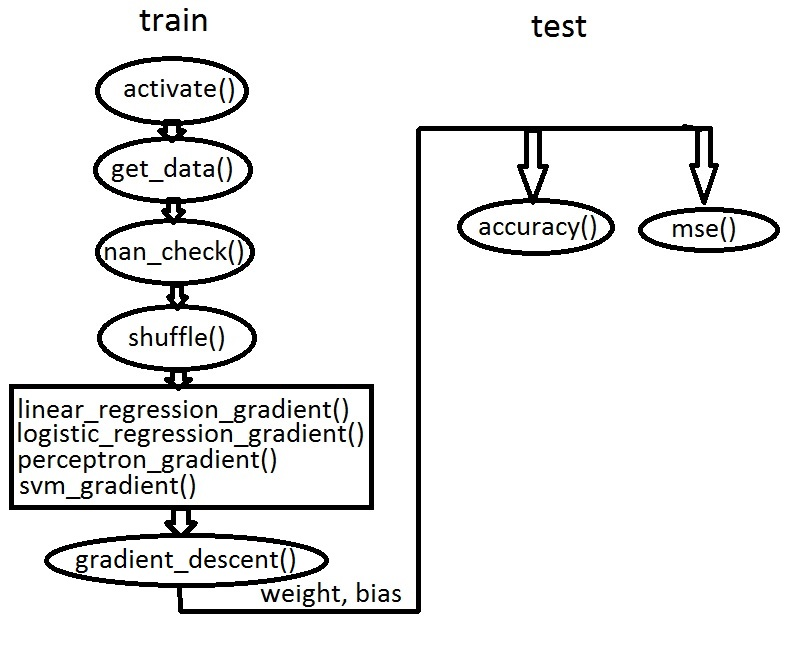
\includegraphics[width = .6\textwidth]{dependencyTree.jpg}


\textbf1.\\
\[\begin{aligned}
\frac{\partial E}{\partial w_j} &= \frac{\partial\sum_{i}\big((t_i-y_i)^2)}{\partial w_j}\\
&=2\sum_i(t_i-y_i)\cdot \frac{\partial\sum_i(t_i-g(w'x_i+b))}{\partial w_j}\\
&=-2\sum_i(t_i-y_i)\cdot g'(w'x_i+b)\cdot x_{i, j}
\end{aligned}\]
\[\begin{aligned}
\frac{\partial E}{db} &= \frac{\partial\sum_{i}\big((t_i-y_i)^2)}{\partial b}\\
&=2\sum_i(t_i-y_i)\cdot \frac{\partial\sum_i(t_i-g(w'x_i+b))}{\partial b}\\
&=-2\sum_i(t_i-y_i) \cdot g'(w'x_i+b) 
\end{aligned}
\]

\textbf2.\\
\[\begin{aligned}
\frac{\partial E}{\partial w_j}&=\frac{\sum_{i}\big((t_i-y_i)^2)}{\partial w_j}\\
&=2\sum_i(t_i-y_i)\cdot \frac{\partial\sum_i(t_i-y_i)}{\partial w_j}\\
&=2\sum_i(t_i-y_i)\cdot \frac{\partial\sum_i(t_i-g(w'x_i+b))}{\partial w_j}\\
&=-2\sum_i(t_i-y_i)\cdot x_{i, j}
\end{aligned}
\]

\textbf3.\\
\[\begin{aligned}
\frac{\partial E}{\partial w_j}&=\frac{\partial\sum_{i}\big((t_i-y_i)^2)}{\partial w_j}\\
&=2\sum_i(t_i-y_i)\cdot \frac{\partial\sum_i(t_i-y_i)}{\partial w_j}\\
&=2\sum_i(t_i-y_i)\cdot \frac{\partial\sum_i(t_i-g(w'x_i+b))}{\partial w_j}\\
&=-2\sum_i(t_i-y_i)\cdot y_i\cdot (1-y_i) \cdot x_{i, j}
\end{aligned}
\]

\textbf4.\\
\[\begin{aligned}
\frac{\partial E}{\partial w_j} &= -\sum_{i:y\neq sign(\vec{w^T}\vec(x))}
\frac{\partial((w'x_i+b)\cdot t_i)}{\partial w_j}\\
&=-\sum_{i:y\neq sign(\vec{w^T}\vec{x})}x_{i, j}\cdot t_j
\end{aligned}
\]

\textbf5.\\
\[\begin{aligned}
\frac{\partial E}{\partial w_j} &= \frac{\partial\|w\|_2^2}{\partial w_j} + C\cdot \sum_{i}\frac{\partial[1-t_i(w'x_i+b)]}{\partial w_j}\\
&=2w_j-C\cdot \sum_{i: y\neq t_i}\frac{d(t_i\cdot (w'x_i + b))}{\partial w_j}\\
&=2w_j-C\cdot \sum_{i: y\neq t_i}t_j\cdot x_{i, j}
\end{aligned}
\]

\section{Code-From-Scratch}
\subsection{Functions}
\textbf{nan\_check(data, label):} \\Find out the nan-rows in datasets and delete these rows\\
\\\textbf{label\_edit(label):} Edit label and change the domain of it from {0, 1} to {-1, 1}\\
\\\textbf{shuffle(data\_set, label\_set):} \\Randomly shuffle the data and label\\
\\\textbf{get\_data(set\_type):} \\Get data from files and storage them in a array. Return the data\_set and label\_set.\\
\\\textbf{linear\_regression\_gradient(data, label, weight, b):} \\Calculate the gradient of linear node classifier. Return the gradient.\\
\\\textbf{logistic\_regression\_gradient(data, label, weight, b):} \\Calculate the gradient of logistic regression . Return the gradient.\\
\\\textbf{perceptron\_gradient(data, label, weight, b = 0):} \\Calculate the gradient of perceptron classifier. Return the gradient.\\
\\\textbf{svm\_gradient(C, data, label, w, b = 0):} \\Calculate the gradient of svm classifier. Return the gradient.\\
\\\textbf{gradient\_descent(weight, b, learning\_rate, gradient\_w = 0, gradient\_b = 0):} \\Update and return weight and b.\\
\\\textbf{compute\_mse(data, label, w, b):} \\Compute the mean square error.\\
\\\textbf{compute\_acc(data, label, w, b):} \\Compute the accuracy\\
\\\textbf{activate(epoch = 2500):} \\Activate the whole neural network and set the iteration as 2500.


\subsection{Lines of codes related to the equations above}

\vspace{10pt}
\textbf1.\\
\[\begin{aligned}
\frac{\partial E}{\partial w_j} &= -2\sum_i(t_i-y_i)\cdot g'(w'x_i+b)\cdot x_{i, j}
\end{aligned}\]
\textbf{Codes: }
\\for i in range(len(label)):
\\gradient\_w -= (-2) * (label[i] - (np.dot(weight, data[i]) + b)) * data[i]
\[\begin{aligned}
\frac{\partial E}{db} &= -2\sum_i(t_i-y_i) \cdot g'(w'x_i+b) 
\end{aligned}\]
\textbf{Codes: }
\\for i in range(len(label)):
\\gradient\_b += (-2) * (label[i] - (np.dot(weight, data[i]) + b))

\vspace{10pt}
\textbf2.\\
\[\begin{aligned}
\frac{\partial E}{\partial w_j}&= -2\sum_i(t_i-y_i)\cdot x_{i, j}
\end{aligned}
\]
\textbf{Codes: }
\\for i in range(len(label)):
\\gradient\_w -= (-2) * (label[i] - (np.dot(weight, data[i]) + b)) * data[i]

\vspace{10pt}
\textbf3.\\
\[\begin{aligned}
\frac{\partial E}{\partial w_j}&= -2\sum_i(t_i-y_i)\cdot y_i\cdot (1-y_i) \cdot x_{i, j}
\end{aligned}
\]
\textbf{Codes: }
\\for i in range(len(label)):
\\gradient\_w += (-2) * ((np.dot(weight, data[i]) + b) - label[i]) * (np.dot(weight, data[i]) + b) * \
                   (1 - (np.dot(weight, data[i]) + b)) * data[i]

\vspace{10pt}
\textbf4.\\
\[\begin{aligned}
\frac{\partial E}{\partial w_j} &= -\sum_{i:y\neq sign(\vec{w^T}\vec{x})}x_{i, j}\cdot t_j
\end{aligned}
\]
\textbf{Codes: }
\\for i in range(len(label)):
\\if np.dot(weight, data[i]) * label[i] < 0 :
\\gradient\_w += (-1) * data[i] * label[i]
\\else:
\\gradient\_w += 0

\vspace{10pt}
\textbf5.\\
\[\begin{aligned}
\frac{\partial E}{\partial w_j} &= 2w_j-C\cdot \sum_{i: y\neq t_i}t_j\cdot x_{i, j}
\end{aligned}
\]
\\\textbf{Codes: }
\\for i in range(len(label)):
\\if label[i] * np.dot(w, data[i]) < 1 :
\\gradient\_w += C * (-1) * data[i] * label[i]
\\gradient\_b += C * (-1) * label[i]
\\else:
\\gradient\_w += 0
\\gradient\_b += 0
\\gradient\_w = (2 * w + gradient\_w) 


\subsection{Results}

\subsubsection{Error Rates Figure}
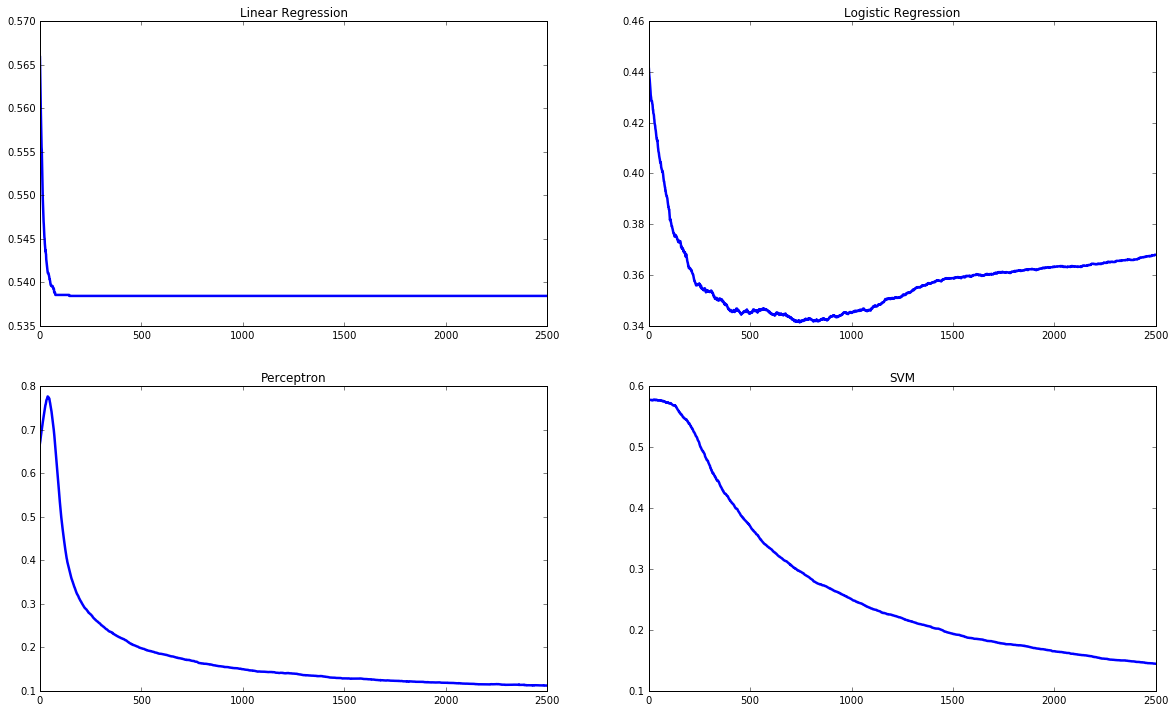
\includegraphics[width = .8\textwidth]{python1.png}

\subsubsection{}
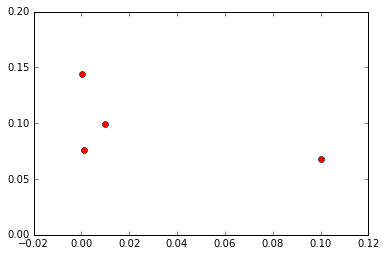
\includegraphics[width = .8\textwidth]{svm_differentC.png}\\
\begin{tabular}{ccc}
\hline
C = 0.1 & C = 0.01& C = 0.001\\
\hline
error rate = 0.068156& 0.099157&0.095678 \\
\hline
\end{tabular}
\begin{tabular}{ccc}
\hline
C = 0.0001\\
\hline
0.144040\\
\hline
\end{tabular}

\subsubsection{Scatter Plot and Different Classifier}
using PCA to reduce the dimensions\\
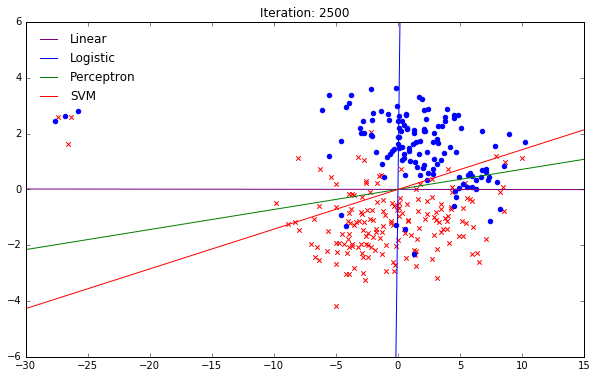
\includegraphics[width = .8\textwidth]{PCA.png}

\section{TensorFlow}
\subsection{Methods}
TensorFlow functions I use and explanations of them are below.\\

\textbf{Codes:}
\\x\_placeholder = tf.placeholder(tf.float32, [None, 16]) 
\\Create a placeholder. For each sample, it has 16 dimensions' feature. When we activate the session, it will input a value.\\

\textbf{Codes:}
\\w = tf.Variable(tf.random\_normal([16, 2])) 
\\creates a variable. It has the shape of [16, 2] because we have 16 features in a sample and we classify it into to classes.
\\\textbf{Codes:}
\\y\_hat = tf.nn.softmax(tf.matmul(x\_placeholder, w) + b) 
\\means we first compute the output by multiply weights and sample, then we use a softmax node to compute the class possibility.
\\\textbf{Codes:}
\\cross\_entropy = tf.reduce\_mean(-tf.reduce\_sum(y\_placeholder * tf.log(y\_hat), reduction
\_indices=[1])) 
\\calculate the cross entropy and the goal of the algorithm is to minimize it. tf.log computes the logarithm of each element, tf.reduce\_mean computes the mean.
\\\textbf{Codes:}
\\correct\_prediction = tf.equal(tf.argmax(y\_hat,1), tf.argmax(y\_placeholder,1)) 
\\finds the correct predictions. tf.argmax finds the index of the highest entry in y\_hat and y\_placeholder and compare if they are the same.
\\\textbf{Codes:}
\\accuracy = tf.reduce\_mean(tf.cast(correct\_prediction, tf.float32)) 
\\tf.cast turn the booleans in correct\_prediction to floating point numbers.\\
\textbf{Codes:}
\\train\_step = tf.train.GradientDescentOptimizer(0.01).minimize(cross\_entropy) 
\\means we choose gradient descent to minimize croos entropy

\textbf{Codes:}
\\init = tf.initialize\_all\_variables() 
\\initializes variables.
\\\textbf{Codes:}
\\sess = tf.Session() 
\\launches the model in a session.
\\\textbf{Codes:}
\\sess.run(init)  
\\input values into variables.

\subsection{Results}
Convergence Figure

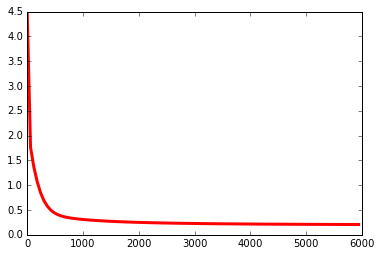
\includegraphics[width = .8\textwidth]{tensor.png}

\rule{0pt}{0pt} 

table 3.1

\begin{tabular}{ccc}
\hline
 & train& eval\\
\hline
error rate& 0.200659& 0.131954\\
\hline
\end{tabular}





















\end{document}